\documentclass[12pt]{article}

%opening
\title{Wielding Constituent Power? The effect of electoral threats on responsiveness and response quality in grassroots policy lobbying}
\author{Joshua Timm \\
PhD Student, University of Southern California}
\usepackage{thmtools}
\usepackage[utf8]{inputenc}
\usepackage[T1]{fontenc}
\usepackage{amsmath,amssymb,amsthm}


\usepackage[english]{babel}
\usepackage{graphicx}
\usepackage{url}
\usepackage{array}
\usepackage{setspace}
\usepackage{graphics}
\usepackage{amssymb}
\usepackage{amsmath}
\usepackage{natbib}
\usepackage{pdflscape}
\usepackage{caption}
\usepackage{fullpage}
\usepackage{multicol}
\usepackage{threeparttable}
%\usepackage{subcaption}
\usepackage{fullpage}
\usepackage{multicol}
\usepackage{threeparttable}
\usepackage{subfig}
\usepackage{multirow}
\usepackage{dcolumn}
\usepackage{setspace}
\doublespacing

\begin{document}

\maketitle


 
\section{Introduction}
This project is largely motivated from observing gun control advocacy efforts after the shootings in Parkland, FL. in February 2018 and Las Vegas in October 2017. After shootings such as these, campaigns urging people to contact their elected representatives to push for gun control legislation appear in response\citep{Henschel:aa, Brinlee:2018aa, SIlverberg:2016aa}. Similarly, counter-advocacy efforts urging people to contact their representatives to block gun control legislation or advance gun rights legislation also appear in response to shootings and gun control advocacy campaigns \citep{Scott-Wong:2018aa, Marans:2018aa}.

I personally know individuals that contacted their representative after the Parkland shooting, advocating for gun control legislation. Curiously, a personal contact told me they actually lied in the email to their representative, fraudulently saying they were a gun owner. When I questioned them on including the lie about gun ownership, they thought the opinions of gun owners had more weight than the opinion of non-gun owners re: the issue of gun control. This behavior led me to question which types of messages in grassroots policy advocacy are more effective than others, and which rhetorical strategies are most effective in grassroots lobbying.\footnote{Throughout the rest of this paper, I will refer to the act of a private individual sending a letter to their representative as "grassroots policy advocacy" or "grassroots lobbying"}
\subsection{Theoretically Motivating the Dependent Variable}
The question of which grassroots lobbying messages are "effective" is problematic for a number of reasons. To begin, a precise definition and operationalization of message "effectiveness" is difficult to achieve. In this case, I would argue that message "effectiveness" is the impact a message has on legislator propensity to vote for legislation or take measures to advance legislation in accordance with that constituent's preferences. Unfortunately, the task of measuring legislator propensity to take legislative action as the result of a single letter, email, call, tweet, etc. is essentially impossible. There are no publicly available indicators of such measures, and even if one was to have intimate personal contact with every legislator in a governing body, I know of no measurable indicators of incremental opinion change or likelihood of voting/taking legislative action to forward a policy.

Instead of measuring message effectiveness, scholars can instead study the concept of representation. The question of which constituents are being represented "more" or "better" than others by their member of Congress is substantively important. Political representation is often measured via proxy of measuring responsiveness and response quality to constituent contact \citep{Butler:2011ac, dahl1956preface,Verba:2003aa}. One of the best and most commonly used methods to study responsiveness and response quality is through audit studies.

However, most existing audit studies mainly study service requests (not policy requests) and the effect of demographic variables such as race/ethnicity (Broockman 2013; Butler and Broockman 2011; Grose, Malhotra, and Van Houweling, 2015; Janusz and Lajevardi, 2016; Mendez 2014), socioeconomic status (Bishin and Hayes 2016; Butler 2014; Carnes and Holbein 2015) or education \cite{Neiman2017}.\footnote{Of course, not all audit studies focus on demographic statistics, see \cite{Grose:2015aa,Costa:2017aa}, but many do.} 

I argue that scholars interested in audit studies should venture to study (1) policy requests over service requests and (2) the effects of various rhetorical strategies on responsiveness and response quality over the effects of demographic variables such as race, ethnicity, and socioeconomic status. (1) It is important to study policy requests in addition to service requests because contacting one's representative to advocate for legislation (a policy request) is one of the primary instruments of democracy. (2) Studying the effects of rhetorical strategies on representation is important because it is well demonstrated by some of the audit studies listed above that representatives are generally less responsive to people of color and lower socioeconomic status.

 In contacting a representative, demographic information can be signaled or indicated through various pieces of information: the name of a constituent can indicate race or ethnicity; vocabulary and spelling can indicate level of education; one's address can signal wealth/socioeconomic status; and other pieces of information can send signals about the identity of a constituent. The substantive importance of this work is found in the fact that people cannot change their race or name, and they cannot easily change their socioeconomic status or address, yet all these factors impact representation. What people \textit{can} alter is how they compose a message to a legislator. For this reason, I believe it is important to study the effects of rhetorical strategy/message composition on representation.
 
 It is important to note that people cannot easily falsify their identity in legislator contact by altering their name to a "white-sounding" name or their address to a wealthier zipcode, even if they had the fairly erudite knowledge that doing so might improve chances of representation. Acquiring the information to contact representatives through official government websites requires people to input their name and address, so to fraudulently contact a representative, one would have to create a fake name and a fake address in that legislator's district. The average person contacting their representative would likely not take these fraudulent steps in honest policy requests. This furthers my argument for the substantive importance of studying how changing message content or rhetorical strategy can effect representation.

%It's understandable that most audit studies examine service requests, as service requests get more responses than policy requests (Butler, Karpowitz and Pope, 2012). Further, not all audit studies are restricted to service requests. For example, some studies consider responsiveness and response quality by matching/mismatching policy preference between constituent and legislator (Grose, Malhotra, and Van Houweling, 2015; Mendez and Grose, 2014). However, given the importance of understanding effectiveness of various types of grassroots lobbying efforts, studying rhetorical strategies is an important area for future scholarship. \\

\section{Theory}
To test the effects of a rhetorical strategy in a policy request on representation, a specific rhetorical strategy must be chosen. For this project I chose to test the effects of threatening to withhold a vote for a representative on responsiveness and response quality.
It is well-documented that legislators are re-election seeking actors. First pioneered by \cite{mayhew1974congress} and \cite{Fenno:1973aa}, later work supports the theory \citep{Fiorina:1974aa}, \citep{Kingdon:1989aa}. The desire to be re-elected is fundamental to the work of members of Congress. Simply enough, a representative cannot accomplish their legislative goals if they are not in office. As a result, much of representatives' behavior is in accordance with the desire to be re-elected. An example of actions in line with re-election seeking behavior is the effort MCs put into handling constituency contact: responding to constituents is an important job that legislators take very seriously \citep{fenno1978home, Frantzich:1986aa, CMF:2011aa}. They use these opportunities for constituency contact to not only learn about constituent opinion and intensity of attitudes, but also to improve their favorability and chances of re-election. This claim is backed up by findings from \cite{Grose:2015aa} that legislators tailor their explanations to constituents in a way that has the effect of causing constituents to believe they are in agreement, even when their policy positions are incongruent. Another work that supports this is \cite{Dropp-Peskowitz2012a}, who show lower rates of responsiveness among representatives with higher electoral victory margins in the previous election.

I ask the question of whether and how much threatening electoral consequences in grassroots lobbying messages effect legislator responsiveness and response quality. I offer a theory of electoral threat-induced responsiveness. The theory's logic is that by directly threatening to withhold a vote for a representative in the context of a policy request, a constituent causes a representative (or more likely a legislative staffer) to prioritize the message over other, non-threatening messages.

%\subsection{Tailored Explanations}
%Based on the work of \cite{Kingdon:1989aa} and \cite{fenno1978home}, \cite{Grose:2015aa} theoretically conceptualize that legislators will explain their discordant or unpopular votes to constituents due to a belief that their constituents will hold them accountable for their voting records. 


\section{Design}
To test the theory of electoral threat-induced responsiveness, a within-subjects design field experiment conducted on members of the House of Representatives is ideal.\footnote{I chose the House of Representatives over the Senate purely for statistical power, rather than theoretical reasons} A within-subjects design allows one to study the effects of a treatment message in a policy request (in this case an electoral threat), compared to a pseudo-control\footnote{For the rest of the paper, I use "pseudo-control" instead of "control" because the message being sent is of course not a true control. A policy request is being sent, but it lacks the specified treatment of an electoral threat.} version of the same policy request. In this design, a single representative would be sent a pseudo-control policy request at one time, and then at a different time be sent a treatment message containing a direct threat to withhold a vote for that representative.

This design allows for replication and expansion of this study with various other possible treatments, beyond the electoral threat message. Ideas for treatment messages in future studies of this type could include a message indicating that the constituent has a personal connection to an issue, or perhaps that the constituent used to agree with the opposite policy position but changed their mind.

Figure 1 below outlines the assignment of treatment groups. For this study, there will be two groups of representatives randomly assigned to only one of two treatment groups. The difference between treatment groups is policy position: representatives in the "Gun Control" treatment group will be sent a message from a constituent advocating for gun control, and representatives in the "Gun Rights" treatment group will be sent a message from a constituent advocating for gun rights.

Each representative in a treatment group will receive an email from a constituent at time one and time two, separated by 45 days\footnote{This amount of time is fairly arbitrary, but it allows a significant amount of time to pass between messages to reduce the chances that any staffer reading the emails would remember an incredibly similarly worded email.}. Further, the order in which a representative receives either a pseudo-control message or an electorally threatening message will be randomized.

The final row of figure 1 lists actual sample sizes for the number of legislators contacted, and in parentheses lists the expected number of responses from those legislators. 217 legislators will be randomly assigned to the Gun Control treatment group, and 218 legislators will be randomly assigned to the Gun Rights treatment group. Based on results from the meta-analysis of audit studies in i\cite{Costa:2017aa}, I expect a response rate of roughly 50\%, or 109 responses from legislators in each group. In terms of number of responses, I expect roughly 218 total responses per treatment group (two letters sent per representative doubles the total amount of responses) and approximately 435 responses total. Again, this assumes about a 50\% response rate per message sent.\\

\begin{figure}[h!]
	\caption{Treatment Assignment}
	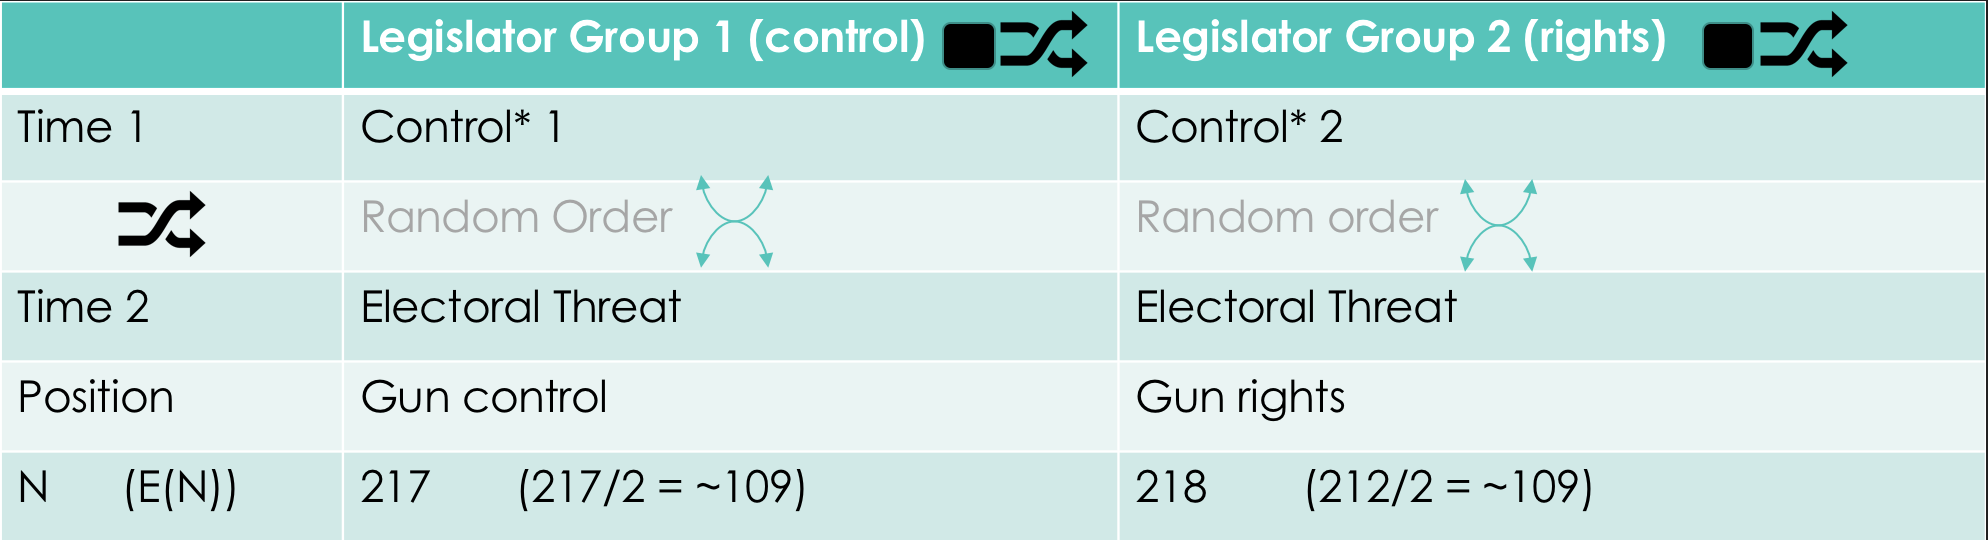
\includegraphics[width=\textwidth]{design_chart.png}\\
\end{figure}

\subsection{Messages}
On the next two pages are samples of what the legislators will be actually be sent. The pseudo-control portion of the text is a general salutation to the congressperson, a paragraph introducing the issue the constituent is writing about, two supporting position-advocacy paragraphs, and a sign-off. The treatment is included at the end of the message in large, bold font with a capitalization at the end. In treatment messages, the bold paragraph will be included, while in pseudo-control messages, the bold paragraph will not be included.\footnote{In one message I only capitalize the word "NOT" and in the other i capitalize "NOT VOTE FOR YOU". As of now, I am undecided on which capitalization method I will actually use. But they will be identical in the final product.}

\begin{figure}[h!]
	\caption{Gun Control Treatment Message}
	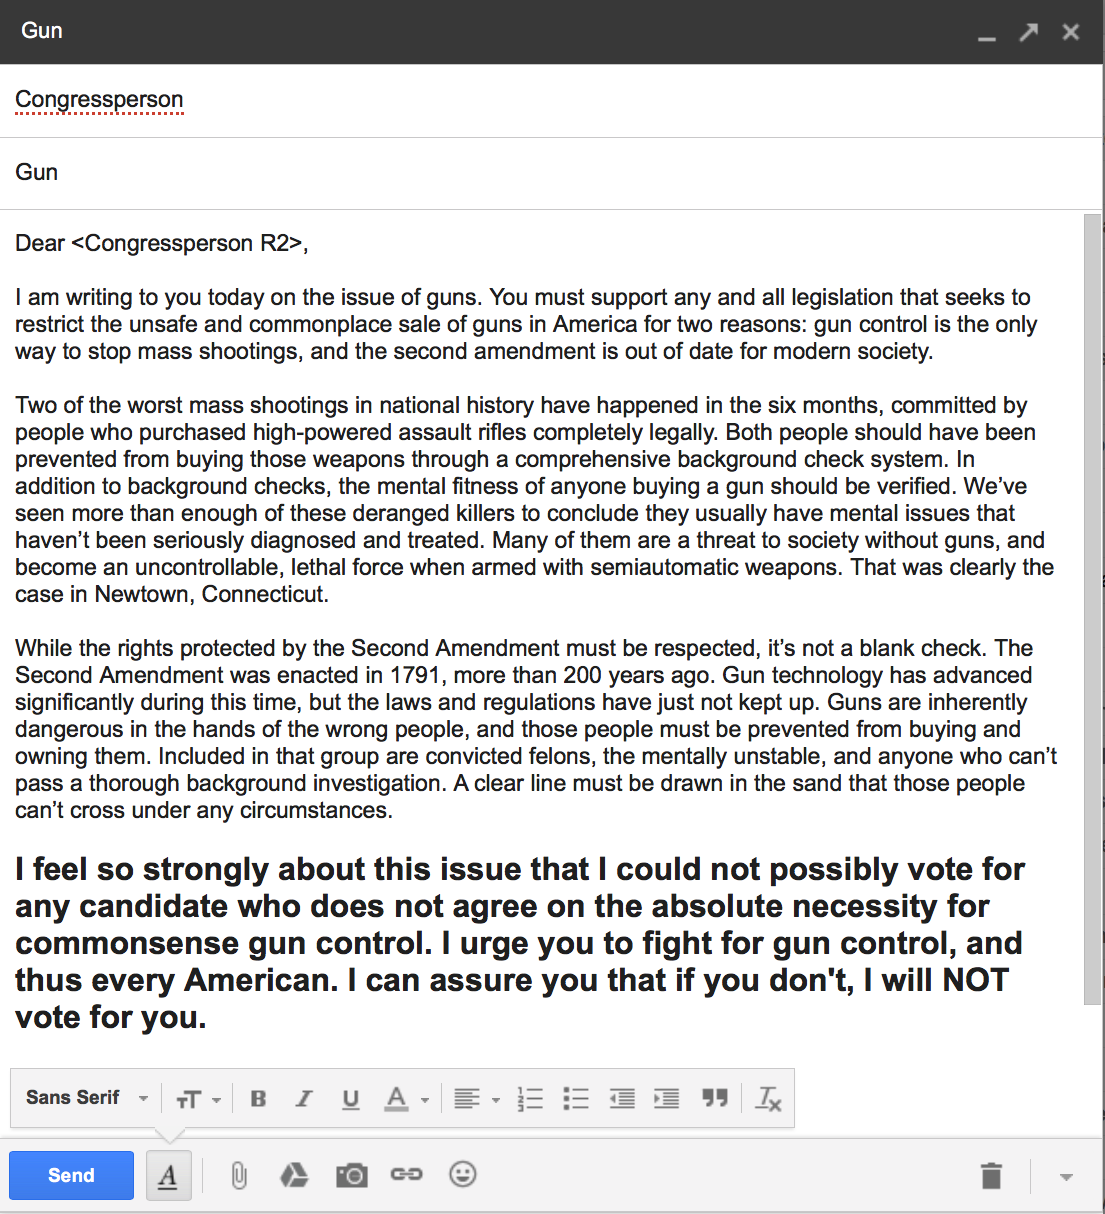
\includegraphics[width=\textwidth]{gun_control.png}
\end{figure}

\begin{figure}[h!]
	\caption{Gun Rights Treatment Message}
	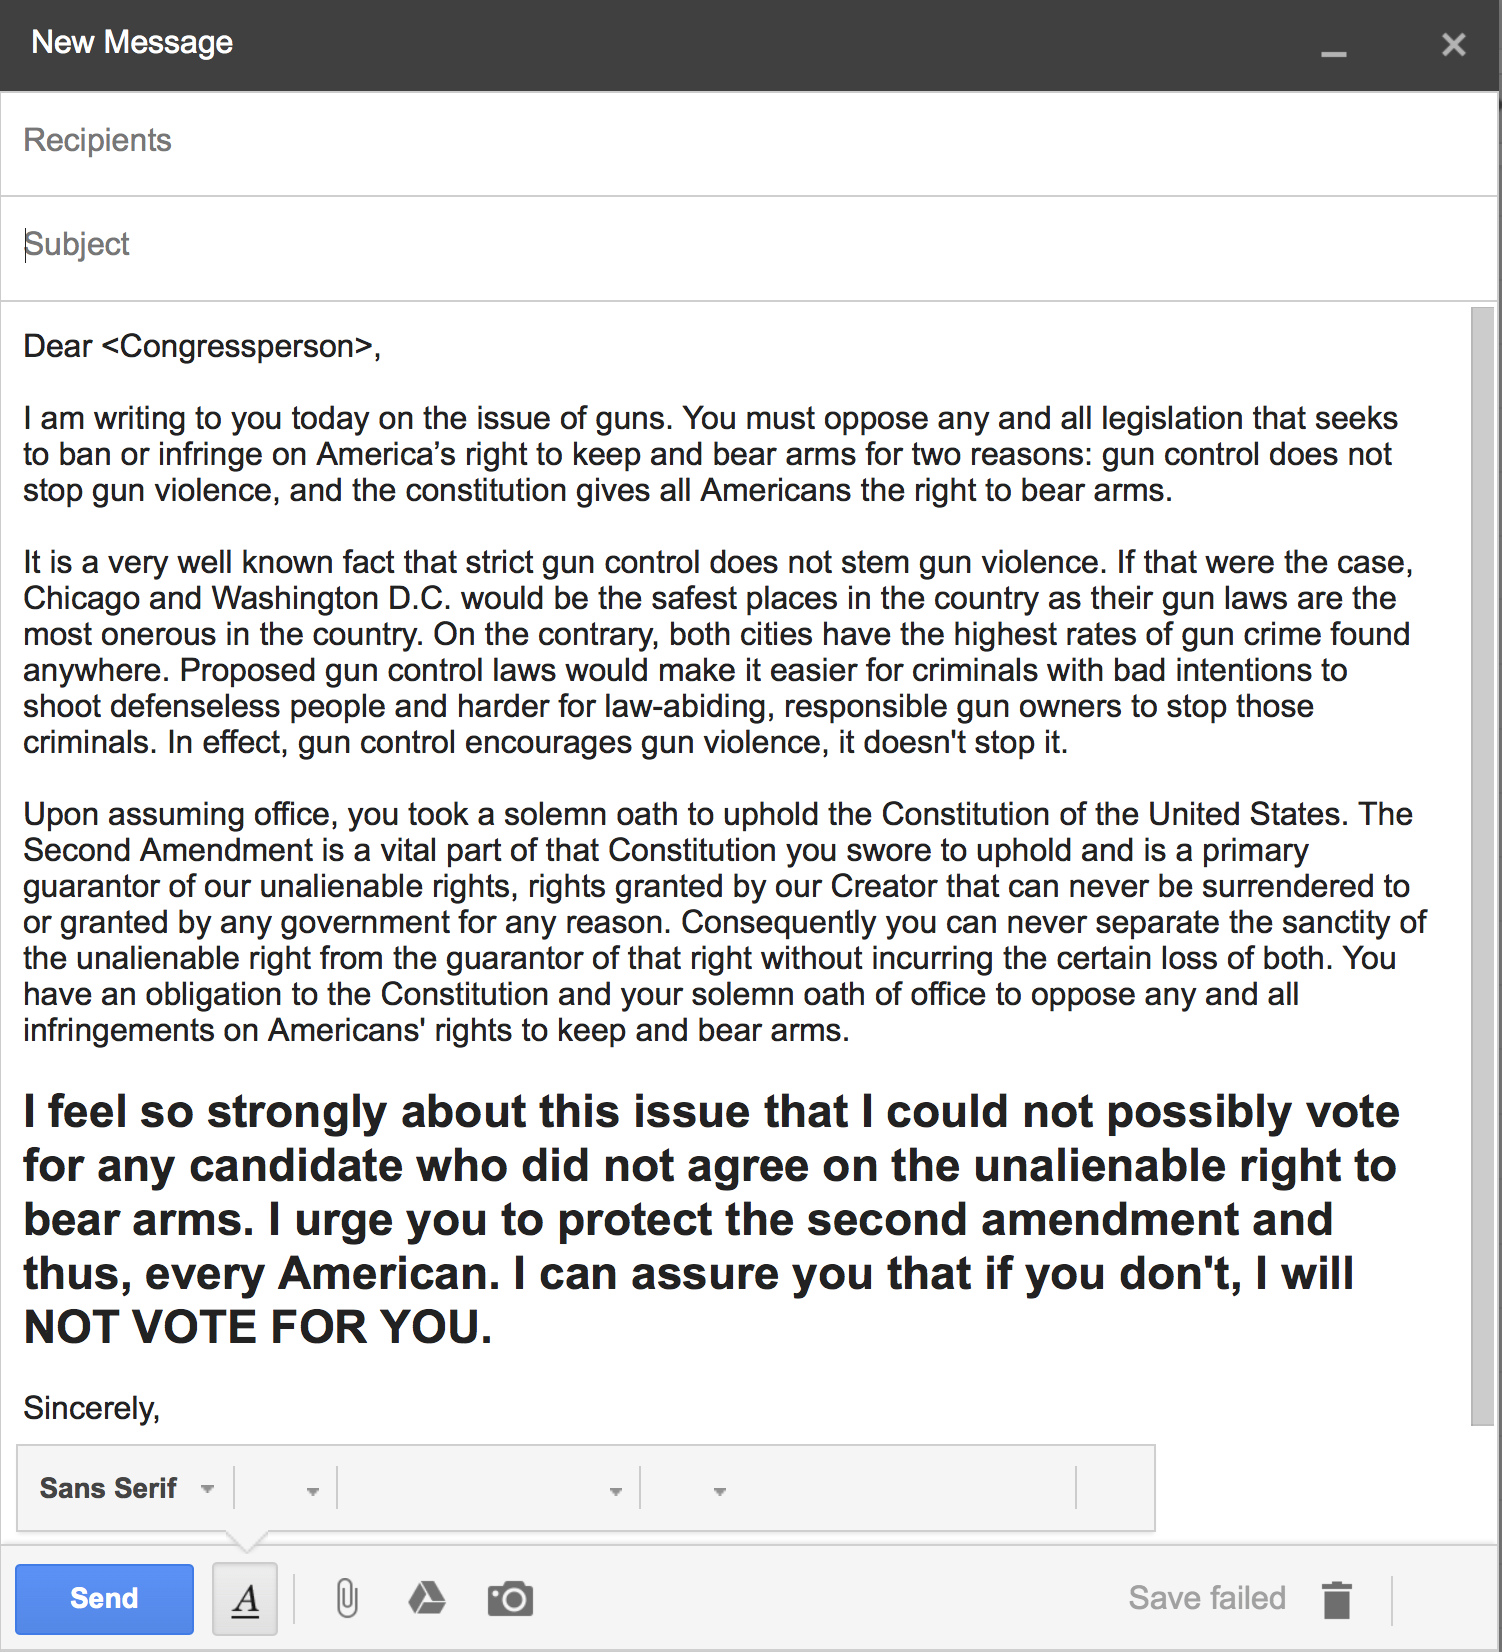
\includegraphics[width=\textwidth]{gun_rights.png}
\end{figure}

\subsection{Observable Implication: Resigning Members}
This year presents a curious opportunity to test an observable implication of the theory. According to \cite{Ballotpedia:2018aa}, 53 members of the US House of Representatives will not be running for re-election in 2018. This allows for a good falsification test for the theory. If representatives are not running for re-election, they face no threats to election. Thus making an electoral threat against a representative should have no effect on responsiveness or response quality. A representative not seeking re-election simply has no greater incentive to respond to an electorally threatening message vs a non electorally-threatening message.

It is possible that a representative might still respond to an electorally threatening constituent's policy request at a greater rate and with higher quality because the treatment message also contains the information that a constituent feels very strongly about an issue. This will be addressed in more detail in the limitations section.

\subsection{Outcome Variables}
The two dependent variables examined in this study are responsiveness and response quality. Responsiveness is defined as how many representatives respond to the constituent, measured in either absolute or percentage amounts. Any message at all will be coded as a response, regardless of the quality of the message. Response Quality will be measured in several ways: length of message; time to respond; inclusion of personal details; and in cases where a representative responds to both messages, if the messages are identical (indicating the treatment itself had no real impact on quality and the policy position was the only important variable). The only two independent variables are the policy position and the electoral threat treatment. In both pseudo-control and treatment messages, a policy request will be made.

\section{Hypotheses}
The theory and design generate several testable hypotheses. Overall, I predict that treatment groups will receive more responses from representatives and that those responses will be of higher quality.

\textbf{Hypothesis 1: }Treatment Groups will receive greater response rate from MCs than Control Groups.

\textbf{Hypothesis 2: }Among MCs that respond to both control and treatment letters, Treatment Group messages will evoke higher response quality from MCs than Control Groups. This hypothesis is weaker than hypothesis 1, and has less of a theoretical drive to it. This also comes with the caveat of hypothesis 2a. 

\textbf{Hypothesis 2a: } Most responses will be the same form letter. Mayhew talked about members of congress writing two "form" letters. One letter to send to constituents with whom they agree on a policy position, and one letter to send to constituents with whom they disagree on a policy position. This is part of a highly professionalized legislative office, where there is not enough time to respond to every form of constituent contact received. It is part of the legislative reality that there simply won't be enough working hours for legislative staffs to tailor messages to each email from each constituent, reading carefully and responding to specific pieces of information in each message. 

\textbf{Hypothesis 3: MCs that disagree with constituent's policy preferences will tailor their explanations to constituents} in accordance with Grose, Malhotra, and Van Houweling 2015's theory of tailored explanations \citep{Kingdon:1989aa,Grose:2015aa,fenno1978home}. They will do this to compensate for policy disagreements while simultaneously attempting to improve support among their constituents.

\subsection{Measuring Representatives' Pre-Treatment Stance on the Issue: Gun Control vs. Gun Rights}
Conducting analysis related to hypothesis 3 requires gathering an existing measure of representative's existing opinions on gun control. This is a non-trivial task because many honest policy requests from constituents will not be about a single clear roll-call vote. The issue of guns in particular is not easily measured by a single roll-call vote. Because of the challenge in measuring issue stance, I have opted to use a measure of gun control position/issue stance developed by the Daily Beast \cite{Michael-Keller:aa}. I chose this measure because it is an up-to-date measure of each representative's stance on gun control as measured by publicly available statements, voting records, ratings from the National Rifle Association and the Brady Campaign to Prevent Gun Violence, and dollar contributions from the gun lobby.

Using this measure, I will include tables that analyze whether the constituent sent a message a representative that either agrees with their position, disagrees with their position, or has an unclear/swing position.


\textbf{Hypothesis 4: No treatment effect will be observed among representatives who are not seeking re-election}\\
If the theory is working as argued, legislators who are not seeking re-election will not have any greater incentive to respond to an electorally threatening message than the control* policy request message. If an effect is observed, I predict it may be due to the treatment message also conveying the information that the constituent holds strong feelings about the issue.

\section{Results}
Because this is an un-implemented design, there are no results to analyze yet. In place of analysis, I include expected results tables. All the numbers are fabricated but should represent values in expected ranges.
% table 1
 \begin{table}[h!]
	\caption{\textbf{Responsiveness among Representatives by Treatment Group}}
	\label{tab2}
	\begin{tabular}{lllllll}
		Responded to Control* Message   && 48\%            &&   47\%\\
		Responded to Treatment Message && 55\%          &&   54\%\\ 
		Difference && 7\%            &&   7\%\\ 
		Responded to Both Messages && 33\% &&   37\%\\
		\hline
		p            && 0.05 				&&   0.05 \\
		N 			 &&      217 			 &&  218    \\
		\hline
		Treatment Group && Gun Control  && Gun Rights & \\
						&&	Letter		&& letter
	\end{tabular}
\end{table}

Table 1 will display basic responsiveness results between the two treatments: the gun control policy request message and the gun rights policy request message. It Shows how many representatives assigned to receive a gun control policy request or a gun rights policy request responded to the control* message, the treatment message, and both messages.

% table 2
 \begin{table}[h!]
	\caption{\textbf{Response Quality Means among Representatives by Treatment Group}}
	\label{tab2}
	\begin{tabular}{lllllll}
		Control* length   && 48\%            &&   47\%\\
		Treatment* length   && 48\%            &&   47\%\\
		Length Difference   && 48\%            &&   47\%\\
		\hline
		Control* Time-to-Respond   && 8            &&   9\\
		Treatment Time-to-Respond && 8          &&   7\\ 
		Time-to-Respond Difference && 1            &&   2\\
		\hline 
		Control* Personal Details                && 7\%            &&   7\% \\
		Treatment Personal Details                && 10\%            &&   10\%\\
		Personal Details Difference && 3\%                      && 3\%\\
		\hline
		p            && 0.05 				&&   0.05 \\
		N 			 &&      217 			 &&  218    \\
		\hline
		Treatment Group && Gun Control  && Gun Rights & \\
		&&	Letter		&& Letter
	\end{tabular}
\end{table}

Table 2 displays the various results of response quality among all representatives, grouped by treatment group assignment. It includes the mean length of responses to the control* message, treatment message, and the difference between the two means; the mean time-to-respond for the control* message, treatment message, and the difference between the two means; the mean rate of inclusion of personal details for the control* message, treatment message, and the difference between the two means.\\
Because representatives who responded to both the control message and treatment letters may be systematically different than representatives who do not, analyses are repeated on these representatives to maintain internal validity. Table 3 below analyses the same response quality variables plus the identical letters variable, but solely on legislators who responded to both letters.

% table 3
 \begin{table}[h!]
	\caption{\textbf{Response quality among Representatives that responded to both letters}}
	\label{tab2}
	\begin{tabular}{lllllll}
		\textbf{Identical Letters}   && \textbf{2\%}           &&   \textbf{3\%} \\
		\hline
	    Control* length   && 48\%            &&   47\%\\
	    Treatment* length   && 48\%            &&   47\%\\
	    Length Difference   && 48\%            &&   47\%\\
	    \hline
	    Control* Time-to-Respond   && 48\%            &&   47\%\\
	    Treatment Time-to-Respond && 55\%          &&   54\%\\ 
	    Time-to-Respond Difference && 7\%            &&   7\%\\ 
	    \hline
	    Control* Personal Details                && 7\%            &&   7\%\\
	    Treatment Personal Details                && 7\%            &&   7\%\\
	    Personal Details Difference && 2\%                      && 2\%\\
	    \hline
	    p            && 0.05 				&&   0.05 \\
	    N 			 &&      50 			 &&  52    \\
	    \hline
	    Treatment Group && Gun Control  && Gun Rights & \\
	    &&	Letter		&& Letter
	\end{tabular}
\end{table}

There may be an external validity problem if results are censored by representatives who only respond to constituents with whom they agree. Thus, analyses are conducted on representatives by the congruence of policy position, using the position of the treatment message and the Daily Beast's measure of each representative's gun control stance. Tables 4 and 5 below analyses responsiveness and response quality, grouping results by whether or not the representative agrees or disagrees with the policy position in the constituent's treatment message. Also included is a group for representatives without a clear stance on gun control/gun rights.

% table 4
\begin{table}[h!]
	\caption{\textbf{Response quality among Representatives that responded to both letters}}
\label{tab2}
\begin{tabular}{lllllll}
	\textbf{Identical Letters }   && \textbf{2\% }           &&   \textbf{3\%}   && \textbf{1\%} \\\\
	\hline
	Responded to Control*   && 45\%            &&   45\%   && 40\% \\
	Responded to Treatment &&   45\%        &&   47\%    && 39\% \\
	Difference                       && 2\%           &&   2\%   && 1\%    \\
	\hline
	p            && 0.05 				&&   0.05 &&  .15\\
	N 			 &&      52 			 &&  46    &&  23\\ 
	\hline
	Sample && Constituent   && Constituent   &&    Unclear/Swing   \\  
	&&								and MC	Agree	&& and MC Disagree               &&   Position\\ 
\end{tabular}
\end{table}

% table 5
 \begin{table}[h!]
	\caption{\textbf{Response quality among Representatives that responded to both letters}}
	\label{tab2}
	\begin{tabular}{lllllll}
		\textbf{Identical Letters}   && \textbf{2\% }           &&   \textbf{3\%}   && \textbf{1\%}\\
		\hline
		Control* length (characters)   && 600            &&   600   && 700 \\
		Treatment* length  (characters) && 700            &&   700   && 700\\
		Length Difference  (characters) && 100           &&   100   && 100\\
		\hline
		Control* Time-to-Respond  (days) && 9            &&   9   && 9\\
		Treatment Time-to-Respond (days) && 7         &&   7    &&  9 \\ 
		Time-to-Respond Difference (days) && 7\%            &&   7\%   &&  9 \\ 
		\hline
		Control* Personal Details                && 20\%            &&   20\%   &&  9\\
		Treatment Personal Details                && 30\%            &&   30\%   &&  9 \\
		Personal Details Difference && .10\%                      &&  10\%   &&  9 \\
		\hline
		p            && 0.05 				&&   0.05 &&  .15\\
		N 			 &&      52 			 &&  46    &&  23\\ 
		\hline
		Sample && Constituent   && Constituent   &&    Unclear/Swing   \\  
		&&								and MC	Agree	&& and MC Disagree               &&   Position\\ 
	\end{tabular}
\end{table}

 

\section{Limitations}
There is some conflation in the electoral threat treatment text. In that text, there are two treatments present (1) how strongly a constituent feels about an issue and (2) a constituent making an electoral threat to a representative. One could argue that perhaps the electoral threat is not the primary treatment being received by a representative, but rather how strongly a constituent feels about an issue. I do not believe it is possible to feasibly isolate these two concepts. If the treatment message does not make an electoral threat, the theory of electoral threat simply isn't being tested. However, there are two issues if the treatment message does not include the "strong feelings about an issue" language: (1) if a constituent says they will not vote for a legislator because of their stance on a single issue, there is a very strong implication that the constituent feels strongly about the issue, so electoral threat cannot be truly isolated from strong feelings; (2) Not including language about 'strong feelings' makes the treatment weaker, and I want to make the treatment very strong to increase responsiveness and N size. Mia Costa's meta-analysis finds average responsiveness among 41 audit studies was only slightly higher than 50\%. Because I will attempt this design with emails, I believe the response rates may be even lower, so it is necessary to keep the treatment quite strong.

\section{Discussion}
In this paper, I generally argue for audit studies to expand their range of focus from demographic-oriented independent variables to more dynamic, rhetorically-oriented independent variables. Specifically, I test the effects of constituents threatening electoral consequences in policy requests and find [results when project actually done]. I argue for the importance of studying different rhetorical strategies in policy requests, because constituents can much more easily change the content of an advocacy message than their name, race, address, or socioeconomic status. 


\bibliographystyle{abbrv}
\bibliography{lit}
\end{document}